\documentclass[11pt,a4paper]{article}

\usepackage[utf8]{inputenc}
\usepackage[T1]{fontenc}
\usepackage{geometry}
\usepackage{titlesec}
\usepackage{graphicx}
\usepackage{float}
\usepackage{xcolor}
\usepackage{listings}
\usepackage{hyperref}
\usepackage{enumitem}

\geometry{margin=2.5cm}

\hypersetup{
    colorlinks=true,
    linkcolor=blue,
    urlcolor=blue
}

\titleformat{\section}
{\large\bfseries}
{\thesection.}{0.5em}{}

\titleformat{\subsection}
{\normalsize\bfseries}
{\thesubsection.}{0.5em}{}

\definecolor{codebg}{rgb}{0.95,0.95,0.95}

\lstset{
    backgroundcolor=\color{codebg},
    basicstyle=\ttfamily\small,
    frame=single,
    breaklines=true,
    columns=fullflexible
}

\begin{document}

\begin{titlepage}
    \centering

    \vspace*{3cm}

    {\Huge \textbf{Benchmarking, Docker, and Load Testing}}\\[1cm]

    {\Large Server Engineering Labs}\\[2cm]

    \textbf{Author:}\\
    Laura Ortiz Moreno\\[1cm]

    \textbf{Topics Covered:}
    \begin{itemize}[leftmargin=4cm]
        \item System benchmarking
        \item ApacheBench load testing
        \item Docker containers
        \item Docker Compose orchestration
        \item JMeter testing
        \item Infrastructure monitoring
    \end{itemize}

    \vfill

    \textbf{Environment:}\\
    Debian Linux Server\\
    Rocky Linux Client VM\\
    Virtualized lab environment

    \vspace{1cm}

\end{titlepage}

\tableofcontents
\newpage

\section{Introduction}

This report documents several benchmarking and infrastructure performance experiments performed in a Linux virtualized environment.

The laboratory focused on:
\begin{itemize}
    \item System benchmarking with Phoronix Test Suite
    \item HTTP load testing with ApacheBench
    \item Containerized deployments using Docker
    \item Multi-container orchestration with Docker Compose
    \item Stress testing using Apache JMeter
    \item Resource monitoring during workload execution
\end{itemize}

The exercises combined benchmarking tools, monitoring systems, and containerized services to simulate realistic server workloads.

\section{Benchmarking Fundamentals}

Two main categories of benchmarking were discussed:
\begin{itemize}
    \item System benchmarking
    \item Service benchmarking
\end{itemize}

The importance of using external clients to perform measurements was emphasized in order to avoid affecting the server under test.

\section{Installing Phoronix Test Suite}

Phoronix Test Suite was installed on the Debian server.

Installation:

\begin{lstlisting}[language=bash]
sudo apt install phoronix-test-suite
\end{lstlisting}

Additional dependencies:

\begin{lstlisting}[language=bash]
sudo apt install curl unzip
\end{lstlisting}

Benchmark execution example:

\begin{lstlisting}[language=bash]
phoronix-test-suite benchmark pts/sudokut
\end{lstlisting}

\begin{figure}[H]
    \centering
    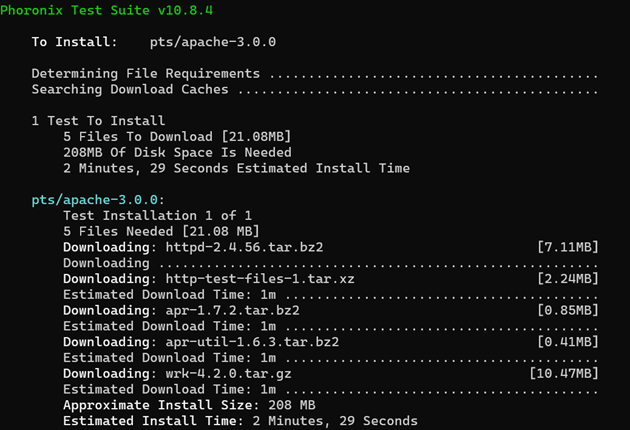
\includegraphics[width=0.82\textwidth]{images/docker-benchmark/phoronix-installation.png}
    \caption{Installation and initialization of the Phoronix Test Suite benchmarking framework.}
\end{figure}

\subsection{Monitoring During Benchmarking}

Resource utilization was monitored during benchmark execution using:
\begin{itemize}
    \item CPU usage
    \item Memory utilization
    \item Service responsiveness
\end{itemize}

\section{HTTP Load Testing with ApacheBench}

ApacheBench (\texttt{ab}) was used to generate concurrent HTTP requests against the server.

Example:

\begin{lstlisting}[language=bash]
ab -n 5000 -c 50 http://server-address/
\end{lstlisting}

Parameters:
\begin{itemize}
    \item \texttt{-n}: total number of requests
    \item \texttt{-c}: concurrency level
\end{itemize}

The tests provided:
\begin{itemize}
    \item Request throughput
    \item Latency statistics
    \item Error rates
    \item Response time percentiles
\end{itemize}

\begin{figure}[H]
    \centering
    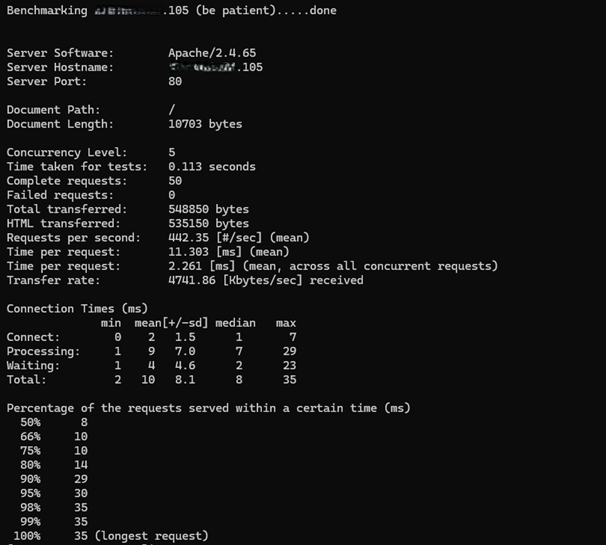
\includegraphics[width=0.90\textwidth]{images/docker-benchmark/apachebench-results.png}
    \caption{ApacheBench performance results showing concurrent request handling and throughput metrics.}
\end{figure}

\section{Docker Fundamentals}

The laboratory introduced containerization concepts using Docker.

Key concepts included:
\begin{itemize}
    \item Images
    \item Containers
    \item Isolation
    \item Lightweight virtualization
\end{itemize}

Docker was installed:

\begin{lstlisting}[language=bash]
sudo apt install docker.io
\end{lstlisting}

Verification:

\begin{lstlisting}[language=bash]
sudo docker ps
\end{lstlisting}

\subsection{Running Containers}

Example container execution:

\begin{lstlisting}[language=bash]
sudo docker run hello-world
\end{lstlisting}

Unused containers and images were cleaned with:

\begin{lstlisting}[language=bash]
sudo docker system prune -a -f
\end{lstlisting}

\section{Docker Compose and Microservices}

Docker Compose was used to orchestrate multiple services simultaneously.

The laboratory included:
\begin{itemize}
    \item Application containers
    \item MongoDB containers
    \item Service orchestration
    \item Resource monitoring
\end{itemize}

Repository cloning example:

\begin{lstlisting}[language=bash]
git clone <repository>
cd application-directory
\end{lstlisting}

Container startup:

\begin{lstlisting}[language=bash]
sudo docker compose up -d
\end{lstlisting}

\begin{figure}[H]
    \centering
    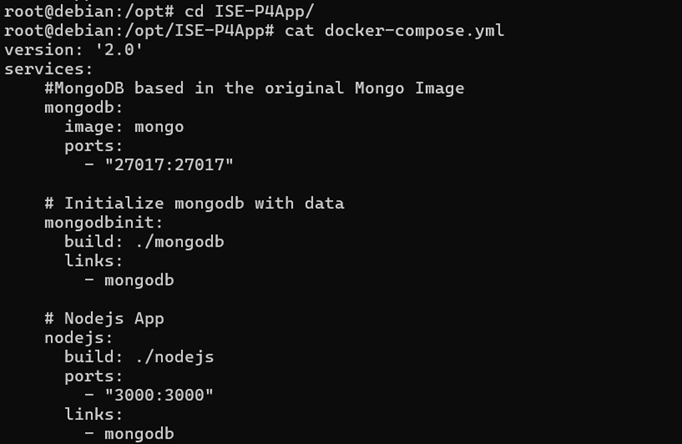
\includegraphics[width=0.88\textwidth]{images/docker-benchmark/docker-compose-config.png}
    \caption{Docker Compose configuration used to orchestrate multi-container application services.}
\end{figure}

\subsection{Monitoring Resource Usage}

Resource utilization was monitored during deployment:
\begin{itemize}
    \item CPU usage
    \item Memory consumption
    \item Container statistics
\end{itemize}

Useful command:

\begin{lstlisting}[language=bash]
docker stats
\end{lstlisting}

\section{Infrastructure Monitoring During Load}

System monitoring was performed during benchmarking and stress tests using Zabbix dashboards.

The monitoring infrastructure allowed visualization of:
\begin{itemize}
    \item CPU spikes
    \item Memory usage
    \item Network activity
    \item System load during stress tests
\end{itemize}

\begin{figure}[H]
    \centering
    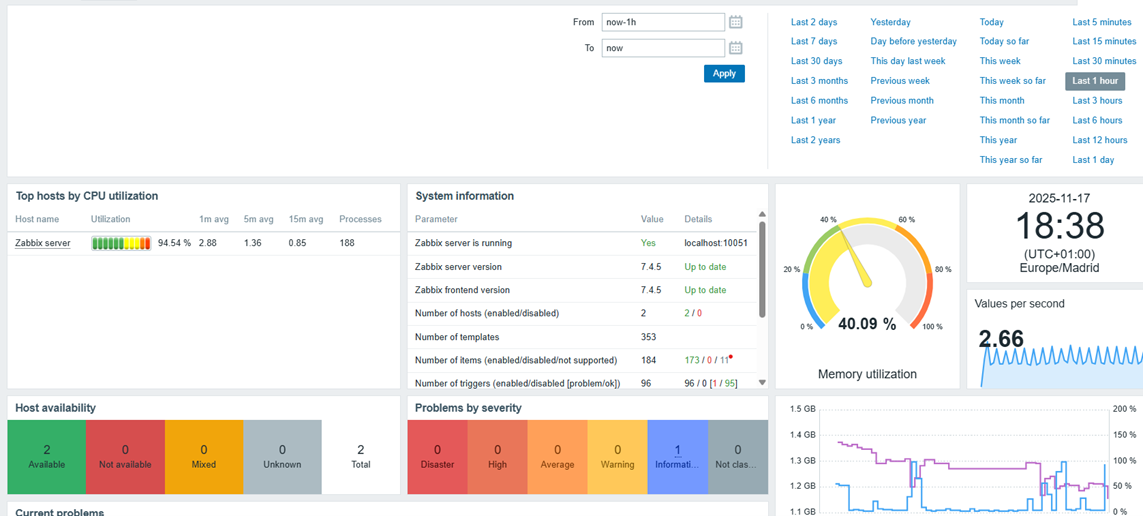
\includegraphics[width=0.94\textwidth]{images/docker-benchmark/zabbix-dashboard-high-load.png}
    \caption{Zabbix dashboard displaying high resource utilization during intensive benchmarking operations.}
\end{figure}

\begin{figure}[H]
    \centering
    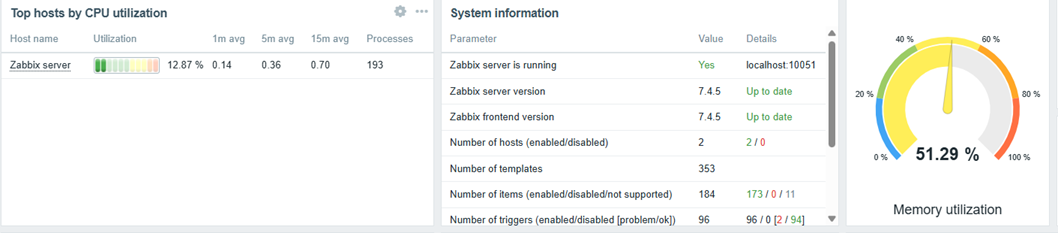
\includegraphics[width=0.94\textwidth]{images/docker-benchmark/zabbix-dashboard-stable.png}
    \caption{System stabilization after load testing with normalized CPU and memory consumption metrics.}
\end{figure}

\section{Load Testing with Apache JMeter}

Apache JMeter was used to simulate concurrent users and API requests.

The tests included:
\begin{itemize}
    \item Login requests
    \item Authenticated API requests
    \item Concurrent user simulation
    \item Performance statistics
\end{itemize}

JMeter execution example:

\begin{lstlisting}[language=bash]
jmeter -n -t test-plan.jmx -l results.jtl
\end{lstlisting}

Parameters:
\begin{itemize}
    \item \texttt{-n}: non-GUI mode
    \item \texttt{-t}: test plan file
    \item \texttt{-l}: output results file
\end{itemize}

\begin{figure}[H]
    \centering
    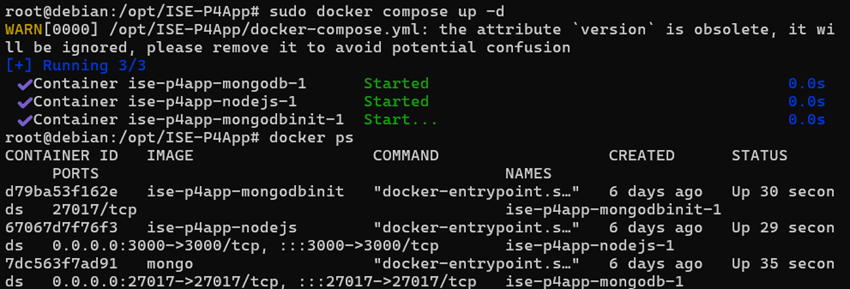
\includegraphics[width=0.90\textwidth]{images/jmeter/docker-compose-running.png}
    \caption{Containerized application stack successfully deployed using Docker Compose prior to load testing.}
\end{figure}

\subsection{API Authentication Testing}

The laboratory also explored:
\begin{itemize}
    \item Basic authentication
    \item Token extraction
    \item Authorization validation
    \item Role-based access testing
\end{itemize}

\begin{figure}[H]
    \centering
    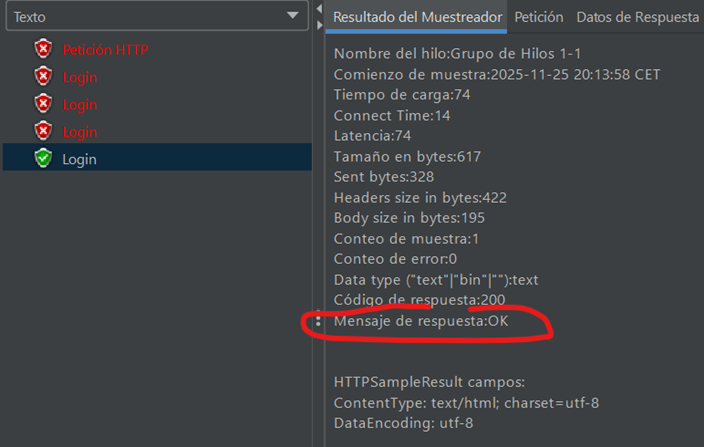
\includegraphics[width=0.78\textwidth]{images/jmeter/jmeter-login-success.png}
    \caption{Successful authentication request executed through Apache JMeter.}
\end{figure}

\begin{figure}[H]
    \centering
    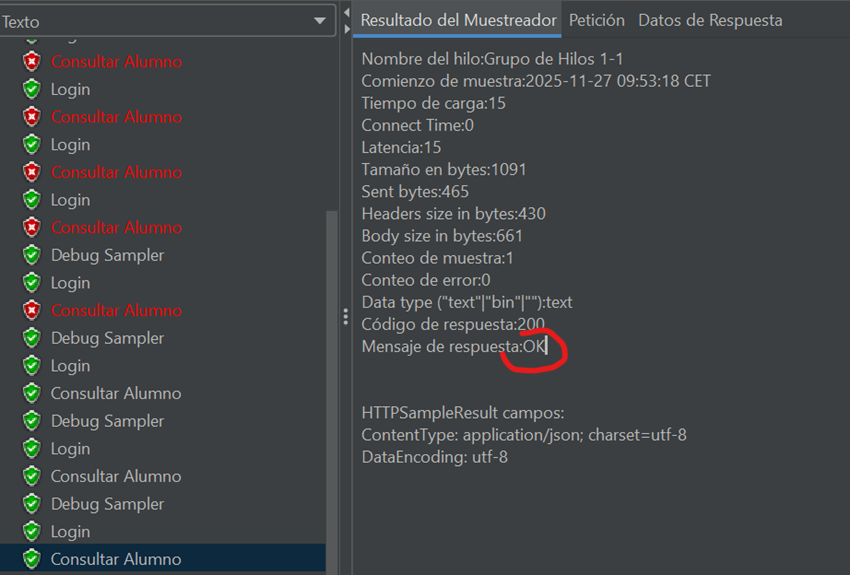
\includegraphics[width=0.84\textwidth]{images/jmeter/jmeter-api-request.png}
    \caption{API request validation performed using authenticated JMeter test scenarios.}
\end{figure}

\subsection{Monitoring Container Performance}

Resource usage during stress testing was monitored directly from Docker.

\begin{figure}[H]
    \centering
    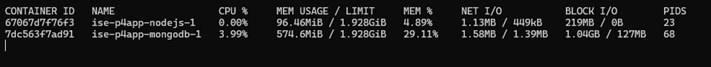
\includegraphics[width=0.92\textwidth]{images/jmeter/docker-resource-monitoring.png}
    \caption{Real-time container resource monitoring using \texttt{docker stats} during concurrent load testing.}
\end{figure}

\subsection{Performance Summary}

JMeter generated aggregated statistics including:
\begin{itemize}
    \item Throughput
    \item Average response time
    \item Error percentage
    \item Request latency
\end{itemize}

\begin{figure}[H]
    \centering
    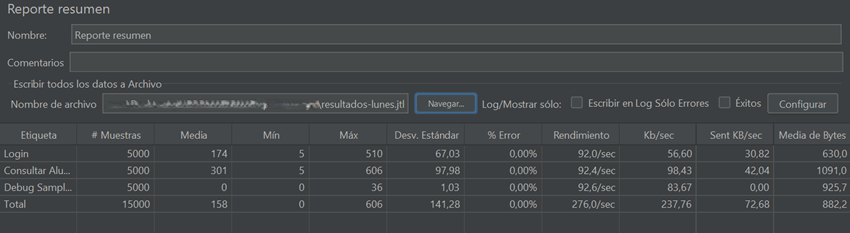
\includegraphics[width=0.88\textwidth]{images/jmeter/jmeter-summary-report.png}
    \caption{Apache JMeter summary report showing aggregated performance metrics under concurrent load conditions.}
\end{figure}

\section{Performance Analysis}

Performance metrics analyzed included:
\begin{itemize}
    \item Throughput
    \item Average response time
    \item Error percentage
    \item Resource utilization
    \item Container performance
\end{itemize}

The monitoring environment allowed observation of CPU and memory behavior under stress conditions.

\section{Challenges Encountered}

Several issues appeared during the laboratory:
\begin{itemize}
    \item Missing package dependencies
    \item Container startup failures
    \item Resource limitations in virtual machines
    \item Incorrect API authentication configuration
    \item High concurrency instability
\end{itemize}

Troubleshooting these problems provided practical experience in infrastructure performance testing.

\section{Conclusion}

This laboratory introduced practical benchmarking and load-testing workflows in Linux infrastructure environments.

The exercises demonstrated:
\begin{itemize}
    \item System benchmarking techniques
    \item Service stress testing
    \item Containerized deployments
    \item Multi-service orchestration
    \item Monitoring under load
    \item API performance validation
\end{itemize}

These concepts are highly relevant in DevOps, backend infrastructure, performance engineering, and cloud-native environments.

\end{document}